
\documentclass[11pt]{article}
\usepackage[margin=0.85in]{geometry}
\usepackage{amsmath,amssymb,amsfonts,amsthm,mathtools}
\usepackage{booktabs,longtable,multirow}
\usepackage{enumitem}
\usepackage{xcolor}
\usepackage{hyperref}
\usepackage{tikz}
\usetikzlibrary{arrows.meta,positioning,fit,calc,shapes.geometric,decorations.pathmorphing}
\usepackage{listings}
\usepackage{microtype}
\usepackage{caption}
\usepackage{graphicx}
\usepackage{subcaption}
\usepackage{float}
\usepackage{needspace}
\usepackage{mathrsfs}
\definecolor{darkblue}{RGB}{25,74,126}
\definecolor{darkgreen}{RGB}{20,112,80}
\definecolor{darkred}{RGB}{143,45,45}
\definecolor{softblue}{RGB}{237,246,255}
\definecolor{softgreen}{RGB}{237,250,244}
\definecolor{softorange}{RGB}{255,247,236}
\definecolor{softpurple}{RGB}{246,241,252}
\definecolor{softyellow}{RGB}{255,252,232}
\definecolor{softslate}{RGB}{247,248,250}
\hypersetup{colorlinks=true, linkcolor=darkblue, citecolor=darkgreen, urlcolor=darkblue}
\lstset{basicstyle=\ttfamily\small,breaklines=true,columns=fullflexible,frame=single,backgroundcolor=\color{softslate}}
\setlist[itemize]{leftmargin=*,itemsep=2pt,topsep=2pt}
\setlist[enumerate]{leftmargin=*,itemsep=2pt,topsep=2pt}
\sloppy

\newtheorem{theorem}{Theorem}[section]
\newtheorem{proposition}[theorem]{Proposition}
\newtheorem{lemma}[theorem]{Lemma}
\newtheorem{corollary}[theorem]{Corollary}
\newtheorem{definition}[theorem]{Definition}
\newtheorem{example}[theorem]{Example}
\newtheorem{remark}[theorem]{Remark}
\newtheorem{assumption}[theorem]{Assumption}

\newcommand{\RR}{\mathbb{R}}
\newcommand{\ZZ}{\mathbb{Z}}
\newcommand{\NN}{\mathbb{N}}
\newcommand{\QQ}{\mathbb{Q}}
\newcommand{\CC}{\mathbb{C}}
\newcommand{\FF}{\mathbb{F}}
\newcommand{\calA}{\mathcal{A}}
\newcommand{\calB}{\mathcal{B}}
\newcommand{\calC}{\mathcal{C}}
\newcommand{\calD}{\mathcal{D}}
\newcommand{\calE}{\mathcal{E}}
\newcommand{\calF}{\mathcal{F}}
\newcommand{\calG}{\mathcal{G}}
\newcommand{\calH}{\mathcal{H}}
\newcommand{\calI}{\mathcal{I}}
\newcommand{\calJ}{\mathcal{J}}
\newcommand{\calK}{\mathcal{K}}
\newcommand{\calL}{\mathcal{L}}
\newcommand{\calM}{\mathcal{M}}
\newcommand{\calN}{\mathcal{N}}
\newcommand{\calO}{\mathcal{O}}
\newcommand{\calP}{\mathcal{P}}
\newcommand{\calQ}{\mathcal{Q}}
\newcommand{\calR}{\mathcal{R}}
\newcommand{\calS}{\mathcal{S}}
\newcommand{\calT}{\mathcal{T}}
\newcommand{\calU}{\mathcal{U}}
\newcommand{\calV}{\mathcal{V}}
\newcommand{\calW}{\mathcal{W}}
\newcommand{\calX}{\mathcal{X}}
\newcommand{\calY}{\mathcal{Y}}
\newcommand{\calZ}{\mathcal{Z}}
\newcommand{\OO}{\mathcal{O}}
\newcommand{\Spec}{\operatorname{Spec}}
\newcommand{\Proj}{\operatorname{Proj}}
\newcommand{\Hom}{\operatorname{Hom}}
\newcommand{\Ext}{\operatorname{Ext}}
\newcommand{\Tor}{\operatorname{Tor}}
\newcommand{\rank}{\operatorname{rank}}
\newcommand{\im}{\operatorname{im}}
\newcommand{\coker}{\operatorname{coker}}
\newcommand{\dist}{\operatorname{dist}}
\newcommand{\diag}{\operatorname{diag}}
\newcommand{\softmax}{\operatorname{softmax}}
\newcommand{\CE}{\operatorname{CE}}
\newcommand{\KL}{\operatorname{KL}}
\newcommand{\Var}{\operatorname{Var}}
\newcommand{\Cov}{\operatorname{Cov}}
\newcommand{\argmax}{\operatorname*{arg\,max}}
\newcommand{\argmin}{\operatorname*{arg\,min}}
\newcommand{\bitsperbyte}{\mathrm{bits\mbox{-}per\mbox{-}byte}}
\newcommand{\loss}{\mathcal{L}}
\newcommand{\eps}{\varepsilon}
\newcommand{\onecone}{one-dimensional cone}
\newcommand{\onecones}{one-dimensional cones}
\numberwithin{equation}{section}

\begin{document}
\begin{titlepage}
\centering
{\Huge\bfseries ToricGT IV:\par}
\vspace{4pt}
{\Huge\bfseries Oracle Trajectory Classifiers for Behavior, Reasoning Quality, and Bits-per-byte Control\par}
\vspace{10pt}
{\Large A NeurIPS-style fourth-iteration research article for ToricGT heads, oracle transformers, trajectory typing, and model-behavior training\par}
\vspace{18pt}
{\large Amelie Schreiber}\par
{\large June 2026}\par
\vfill
\begin{abstract}
ToricGT I made toric geometry operational for graph-token reasoning by turning cones, normal fans, affine semigroups, BGG/Koszul certificates, Gale duality, toric ideals, and GraphCG behavior corridors into finite train-time supervision. ToricGT II made the object dynamical: a reasoning step became a standardized packet whose filtered simplicial complex, multigraded persistence module, derived object, sheaf, vector bundle, differential-form features, and toric chart codes evolve under repeated learned graph-to-graph updates. ToricGT III moved the same framework outside the model into model-context protocols, markdown memory, knowledge graphs, graph-structured vector databases, projected retrieval heads, quantized toric context codes, and long 1--10M-token iterative context windows driven by tropical ring attention.

ToricGT IV adds an oracle layer. The goal is to train either an additional classifier head on top of an existing reasoning model or a full oracle transformer that classifies completed and partial reasoning trajectories into structured behavioral, epistemic, computational, and stylistic types: accuracy, faithfulness, evidence grounding, tool discipline, compliance, safety, refusal appropriateness, tone, personality corridor, verbosity, proof rigor, uncertainty calibration, efficiency, retrieval hygiene, memory hygiene, and graph-of-thought compositionality. The oracle is not a post hoc sentiment classifier. It is a mathematically constrained trajectory-type model whose outputs live in a property poset, a Stanley-Reisner compatibility complex, a toric property fan, a multigraded label module, and a sheaf of local-window judgments. It can be trained as a lightweight head, a frozen-backbone probe, a low-rank adapter stack, or a full transformer over graph-structured trajectory packets.

We develop a rigorous theory of oracle trajectory classification. We define trajectory objects, property lattices, behavior sheaves, toric property polytopes, persistence-label modules, derived residuals, and calibrated multi-label distributions. We prove equivariance, proper-scoring, side-information, isotonic projection, sheaf-gluing, persistence-stability, toric-margin, oracle-guided policy-improvement, and ergodic-occupancy theorems. We then give a concrete training paradigm: label acquisition, weak supervision, verifier distillation, human/rubric calibration, contrastive trajectory pairs, bits-per-byte-gated promotion, oracle-assisted reinforcement or preference training, GFlowNet reward shaping, retrieval filtering, memory pruning, MCP tool-call gating, and test-time behavior projection. The guiding principle is unchanged: the oracle exists to improve model behavior and reasoning, not to decorate the system with attractive mathematics. A trajectory label is useful only when it predicts future bytes, improves answer quality, reduces error, improves controllability, or prevents a costly failure under auditable deployment constraints.
\end{abstract}
\vfill
\begin{minipage}{0.92\textwidth}
\textbf{Design contract.} ToricGT IV treats behavior as a property of reasoning trajectories, not merely final logits. The oracle reads graph-of-thought packets, MCP/memory/KG context events, filtered complexes, certificate signatures, verifier traces, and output drafts. It emits calibrated property distributions and certified incompatibility warnings. Those signals are used to improve training only through score-safe, ablated channels: supervised loss weighting, rejection sampling, preference optimization, reward shaping, retrieval gating, memory hygiene, or lightweight steering. Anything that improves the oracle but worsens held-out bits-per-byte, verified task quality, or artifact efficiency remains teacher-side.
\end{minipage}
\end{titlepage}
\tableofcontents
\clearpage

\section{Purpose and continuity with ToricGT I--III}
\subsection{The fourth problem}
The first three ToricGT papers progressively enlarge the object of supervision. ToricGT I supervises graph-token reasoning with finite toric, tropical, BGG, Koszul, Gale-dual, and behavior-corridor certificates. ToricGT II studies iterative reasoning dynamics by attaching filtered simplicial complexes, multigraded persistence modules, sheaves, vector bundles, differential forms, derived objects, and ergodic summaries to each reasoning step. ToricGT III embeds the same machinery in the external memory substrate: model-context protocols, markdown memory, knowledge graphs, projected graph-structured vector databases, quantized retrieval codes, and 1--10M-token long-context tropical ring attention.

ToricGT IV asks a different but necessary question. Suppose the model can construct rich reasoning trajectories. Which trajectories are good? Which are accurate, efficient, compliant, well calibrated, grounded, concise, rigorous, or stable in tone? Which ones are unsafe, hallucinated, overconfident, sycophantic, evasive, too verbose, too terse, tool-abusive, memory-leaky, or brittle? A base language-model loss sees only bytes. A verifier sees only a task slice. A safety classifier often sees only a final answer. A useful reasoning agent needs a \\emph{trajectory oracle}: a trainable model that classifies the entire trajectory, including hidden graph-of-thought structure, context assembly, memory retrieval, tool use, proof obligations, verifier traces, and final response properties.

The ToricGT IV thesis is:
\begin{quote}
A trajectory classifier becomes useful for training reasoning agents when its labels are structured enough to be compositional, local-to-global, calibrated, compatible with graph symmetries, and predictive of downstream log score, reasoning quality, or behavior reliability.
\end{quote}
The classifier may be a small additional head on an existing ToricGT backbone, or a full oracle transformer trained on trajectory packets. The head is cheaper and easier to ablate; the full oracle is more expressive and can be used as a teacher, dataset judge, and training-time reward model.

\subsection{Relation to ToricGT I}
ToricGT I introduced a graph-token model family
\begin{equation}
F_\theta = D\circ \Phi_L\circ\cdots\circ\Phi_1\circ T,
\end{equation}
where $T$ tokenizes typed graphs, the blocks $\Phi_\ell$ are permutation-equivariant over node and edge tokens, and $D$ decodes graph, node, edge, or byte-level outputs. Its toric layer is a finite-certification layer: tropical active faces, Newton-polytope cells, toric ideals, Cox degrees, BGG differentials, Gale-dual labels, and Euler-Koszul certificates organize hidden states without forcing a deployed byte model to carry a full symbolic algebra system.

ToricGT IV uses the same finite-certification layer as an oracle input. A classifier that sees only final text cannot distinguish a correct answer obtained from a stable proof from a lucky answer obtained by hallucinated intermediate reasoning. A trajectory oracle can classify the proof skeleton, hidden certificate residuals, evidence path, and behavior-corridor occupancy. It therefore supplies a richer target for improving the base model.

\subsection{Relation to ToricGT II}
ToricGT II replaced isolated certificates by dynamical objects. A reasoning step $x_t$ induces a filtered complex $\calK_t$, a persistence module $\calM_t$, a derived object $\calD_t$, a sheaf/vector-bundle object $\calF_t$, differential-form features $\omega_t$, and a toric chart code $c_t$. Repeated application of a learned graph-to-graph map produces
\begin{equation}
(x_0,\calK_0,\calM_0,\calD_0,\calF_0,c_0)\to (x_1,\calK_1,\calM_1,\calD_1,\calF_1,c_1)\to\cdots.
\end{equation}
ToricGT IV classifies this sequence. Instead of using Betti drift, sheaf gluing, or ergodic occupation only as auxiliary metrics, we treat them as features and sometimes labels. A trajectory type can include ``stable persistence'', ``late evidence collapse'', ``refusal boundary crossing'', ``proof branch merged coherently'', or ``tone drift after memory retrieval''.

\subsection{Relation to ToricGT III}
ToricGT III externalized the trajectory into the context substrate. Model-context-protocol calls, markdown memory blocks, knowledge-graph neighborhoods, tool/resource/prompt records, and long-context windows become typed graph objects. ToricGT IV adds an oracle that reads those context events and predicts properties of the resulting reasoning trajectory. For example, the oracle may decide that a tool-call plan is accurate but inefficient, that retrieved memory is relevant but stale, that a citation block is grounded but too verbose, or that a long-context fill policy is likely to exceed the marginal utility threshold.

The official model-context-protocol specification treats MCP as a protocol connecting LLM applications to external data sources and tools, with server features such as tools, resources, and prompts. ToricGT III treats those protocol events as graph-structured retrieval objects; ToricGT IV treats them as oracle-classification evidence for tool discipline, permission safety, grounding, memory hygiene, and answer reliability \cite{mcp2025}.

\subsection{Contributions}
\begin{enumerate}
\item We formalize a trajectory property space containing accuracy, tone, personality, compliance, safety, efficiency, evidence grounding, reasoning quality, tool discipline, retrieval hygiene, memory hygiene, and output-style properties.
\item We define two oracle architectures: a low-cost trajectory-classifier head on the base model and a full oracle transformer over graph-structured trajectory packets.
\item We impose mathematical structure on labels: property posets, Stanley-Reisner compatibility complexes, toric property polytopes, multigraded label modules, Cech-style local-to-global gluing, persistence stability, and derived residual certificates.
\item We prove core theorems that justify using oracle outputs to improve training: equivariance, proper scoring, side-information bounds for bits-per-byte, isotonic projection, sheaf gluing, stability under persistence perturbations, margin-preserving quantization, oracle-guided policy improvement, and ergodic control.
\item We give a concrete training paradigm: dataset construction, label sourcing, verifier distillation, human calibration, weak supervision, frozen-probe training, adapter training, full-oracle training, oracle distillation into the base model, and deployment gating.
\item We specify how oracle labels improve the base model through supervised fine-tuning, preference optimization, GFlowNet rewards, trajectory rejection, retrieval and memory filtering, context-window planning, MCP tool-call gating, and low-rank behavior projection.
\end{enumerate}

\begin{figure}[!htbp]
\centering
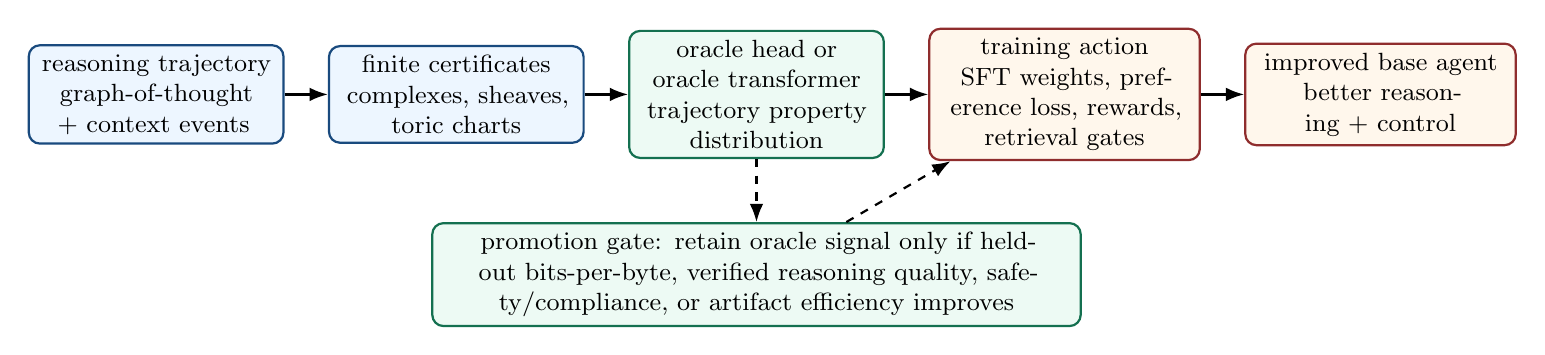
\begin{tikzpicture}[font=\small, node distance=0.55cm, >=Latex]
\tikzstyle{box}=[rounded corners, draw=darkblue, thick, fill=softblue, minimum height=0.9cm, text width=3.0cm, align=center]
\tikzstyle{gbox}=[rounded corners, draw=darkgreen, thick, fill=softgreen, minimum height=0.9cm, text width=3.0cm, align=center]
\tikzstyle{obox}=[rounded corners, draw=darkred, thick, fill=softorange, minimum height=0.9cm, text width=3.2cm, align=center]
\node[box] (traj) {reasoning trajectory\\graph-of-thought + context events};
\node[box, right=0.55cm of traj] (cert) {finite certificates\\complexes, sheaves, toric charts};
\node[gbox, right=0.55cm of cert] (oracle) {oracle head or oracle transformer\\trajectory property distribution};
\node[obox, right=0.55cm of oracle] (train) {training action\\SFT weights, preference loss, rewards, retrieval gates};
\node[obox, right=0.55cm of train] (base) {improved base agent\\better reasoning + control};
\draw[->, thick] (traj) -- (cert);
\draw[->, thick] (cert) -- (oracle);
\draw[->, thick] (oracle) -- (train);
\draw[->, thick] (train) -- (base);
\node[gbox, below=0.8cm of oracle, text width=8.0cm] (gate) {promotion gate: retain oracle signal only if held-out bits-per-byte, verified reasoning quality, safety/compliance, or artifact efficiency improves};
\draw[->, thick, dashed] (oracle) -- (gate);
\draw[->, thick, dashed] (gate) -- (train);
\end{tikzpicture}
\caption{ToricGT IV system view. The oracle reads complete or partial trajectory packets plus finite ToricGT certificates, emits calibrated property distributions, and influences training only through auditable channels.}
\label{fig:tgt4-system}
\end{figure}

\section{The trajectory object and its property space}
\subsection{Trajectory packets}
\begin{definition}[ToricGT trajectory packet]
Fix a horizon $T$, padding sizes, and finite type vocabularies. A ToricGT trajectory packet is
\begin{equation}
\tau = (G_\tau, X_{0:T}, C_{0:T}, R_{0:T}, V_{0:T}, Y, B_{<T}),
\end{equation}
where $G_\tau=(V_\tau,E_\tau)$ is a directed acyclic graph-of-thought topology; $X_t$ is the standardized reasoning-step tensor at vertex or time $t$; $C_t$ contains certificate objects; $R_t$ contains retrieval/memory/MCP event summaries; $V_t$ contains verifier, evidence, and tool-return fields; $Y$ is the final response or intermediate output; and $B_{<T}$ is the strict byte prefix available before scoring the relevant output bytes.
\end{definition}

The packet is deliberately redundant. A classifier head may use only hidden states and a few summaries. A full oracle transformer may use the whole packet, including graph edges, certificate matrices, Cech overlaps, retrieved knowledge-graph paths, and long-context blocks. Redundancy helps with auditability: if the oracle says ``low grounding'', one should be able to inspect whether the cause is missing evidence, stale memory, unsupported tool output, or a failed gluing condition.

\begin{definition}[Certificate field]
A certificate field attached to a trajectory packet is a tuple
\begin{equation}
C_t=(\calK_t,\calM_t,\calD_t,\calF_t,\omega_t,\Sigma_t,\beta_t,\gamma_t),
\end{equation}
where $\calK_t$ is a filtered simplicial complex, $\calM_t$ is a multigraded persistence module, $\calD_t$ is a bounded derived object or a finite chain complex representative, $\calF_t$ is a sheaf/vector-bundle object over a local cover, $\omega_t$ is a differential-form feature, $\Sigma_t$ is a toric fan or occupied empirical fan, $\beta_t$ is a Betti or barcode summary, and $\gamma_t$ stores Cox degrees, one-dimensional-cone activations, tableaux/crystal labels, or root-system chamber codes.
\end{definition}

\subsection{Atomic properties}
A trajectory oracle should classify more than ``good'' or ``bad''. The property set must be broad enough to support targeted improvement and narrow enough to be learnable.

\begin{definition}[Atomic trajectory property]
An atomic trajectory property is a tuple
\begin{equation}
p=(\mathrm{name},\mathrm{scope},\mathrm{polarity},\mathrm{scale},\mathrm{evidence\_rule},\mathrm{action\_rule}).
\end{equation}
The scope is one of token, step, branch, tool call, memory retrieval, proof obligation, final answer, or whole trajectory. The polarity indicates desirable, undesirable, neutral, or context-dependent status. The scale is binary, ordinal, continuous, distributional, or set-valued. The evidence rule states what finite information can support the label. The action rule states how the training system may use the label.
\end{definition}

Core property families include:
\begin{enumerate}
\item \textbf{Epistemic properties:} factual accuracy, mathematical correctness, uncertainty calibration, citation adequacy, evidence grounding, verifier agreement, contradiction risk.
\item \textbf{Reasoning properties:} decomposition quality, proof rigor, branch usefulness, merge consistency, persistence stability, derived residual, algebraic certificate validity, root-system/tableau normal-form correctness.
\item \textbf{Efficiency properties:} context economy, tool-call economy, retrieval precision, token budget discipline, latency estimate, bits-per-byte utility, artifact-byte utility.
\item \textbf{Behavior properties:} compliance with user intent, safety boundary handling, refusal appropriateness, safe-alternative quality, tone, personality corridor, verbosity, empathy, confidence, domain register.
\item \textbf{Memory and MCP properties:} permission correctness, stale-memory risk, memory contamination, KG neighborhood relevance, tool schema compliance, resource provenance, markdown section hygiene.
\end{enumerate}

\subsection{Property posets and compatibility complexes}
Many properties are ordered. ``Fully grounded'' implies ``partially grounded''; ``severe hallucination'' implies ``unsupported claim''; ``unsafe compliance'' is incompatible with ``safe refusal'' but may coexist with ``polite tone''. We encode this explicitly.

\begin{definition}[Property poset]
Let $\calP$ be a finite set of atomic properties. A property poset is a partial order $(\calP,\preceq)$ where $p\preceq q$ means that property $q$ entails property $p$. A label vector $y\in\{0,1\}^{\calP}$ is upward-consistent if $y_q=1$ and $p\preceq q$ imply $y_p=1$.
\end{definition}

\begin{definition}[Compatibility complex]
A compatibility complex is an abstract simplicial complex $\Delta\subseteq 2^{\calP}$. A set $S\subseteq\calP$ is admissible if $S\in\Delta$. Minimal nonfaces encode forbidden coactivations, such as high confidence with no evidence, unsafe tool use with compliance approval, or verbose style with low token budget when concise answer is required.
\end{definition}

The Stanley-Reisner ideal of $\Delta$ is
\begin{equation}
I_\Delta=\left\langle \prod_{p\in F} z_p : F\notin\Delta\right\rangle \subset k[z_p:p\in\calP].
\end{equation}
For soft labels $\hat y_p\in[0,1]$, the differentiable nonface penalty is
\begin{equation}
\loss_{\mathrm{SR}}(\hat y)=\sum_{F\in \mathrm{MinNonFaces}(\Delta)} w_F\prod_{p\in F}\hat y_p.
\end{equation}
This is a compact algebraic way to prevent incompatible behavior labels from being simultaneously high.

\subsection{Toric property polytopes}
\begin{definition}[Toric property polytope]
Choose an embedding $a_p\in M$ for every atomic property $p\in\calP$. The property polytope is
\begin{equation}
P_{\calP}=\mathrm{Conv}\{a_p:p\in\calP\}\subset M_\RR.
\end{equation}
Given oracle logits $\ell_p(\tau)$, the tropical property score is
\begin{equation}
\psi(\tau)=\max_{p\in\calP}\{\ell_p(\tau)\}.
\end{equation}
The active property face is the set of properties whose logits attain or nearly attain the maximum. Its normal-fan cone is the local behavior type of the trajectory.
\end{definition}

The purpose of the toric polytope is not decorative. It gives an audit for classifier decisions. If two properties share an edge in $P_\calP$, they are expected to exchange under small perturbations; if they are separated by many facets, a sudden swap suggests instability. One-dimensional cones of the normal fan become interpretable axes: evidence support, refusal strength, proof rigor, warmth, verbosity, tool reliance, and uncertainty.

\begin{definition}[Property fan margin]
Let $r^\star=\argmax_p\ell_p(\tau)$ be unique. The unnormalized property fan margin is
\begin{equation}
\Delta_{\calP}(\tau)=\min_{q\ne r^\star}\bigl(\ell_{r^\star}(\tau)-\ell_q(\tau)\bigr).
\end{equation}
For grouped or multi-label properties, replace the singleton $r^\star$ by the active face and take the minimum gap to inactive competitors.
\end{definition}

Large margins are useful because they make oracle labels robust to quantization, adapter perturbations, and context-window compression.

\section{Oracle architectures}
\subsection{Additional oracle head}
The cheapest implementation is a classifier head on top of an existing ToricGT or transformer backbone. Let $H_\theta(\tau)$ denote hidden trajectory features: pooled graph-token states, final hidden states, certificate summaries, retrieved evidence features, and output-draft features. An oracle head is
\begin{equation}
O_\phi(\tau)=\bigl(q_\phi(y_p=1\mid \tau)\bigr)_{p\in\calP},
\end{equation}
with optional ordinal, continuous, or distributional outputs.

A lightweight head should be used first because it tests whether the base representation already contains property information. If a frozen head cannot learn useful trajectory labels, the base model likely lacks the needed internal structure or the labels are too noisy. If a frozen head performs well, then training the base model with the oracle signal is safer.

\subsection{Full oracle transformer}
A full oracle transformer is a separate model $\Omega_\psi$ that reads trajectory packets directly. Its input tokens include:
\begin{enumerate}
\item step tokens: hidden-state summaries, output text chunks, verifier scores, evidence vectors;
\item graph tokens: branch/merge edges, tool-call edges, retrieval edges, memory-update edges;
\item certificate tokens: boundary matrices, Betti tables, barcode summaries, Cox degrees, one-dimensional-cone occupancies, tableaux, root-system chamber labels;
\item context tokens: MCP events, markdown blocks, KG triples, source identifiers, permissions, freshness, and provenance;
\item response tokens: final answer draft, citations, refusal text, or structured output.
\end{enumerate}
The full oracle can use ordinary attention, tropical ring attention, projected retrieval into the ToricGT III graph-structured vector database, and local certificate computation.

\begin{definition}[Oracle transformer]
An oracle transformer is a map
\begin{equation}
\Omega_\psi:\calT\to \prod_{p\in\calP}\calY_p
\end{equation}
from the space $\calT$ of bounded trajectory packets to property-output spaces $\calY_p$. It is graph-invariant if relabeling graph-of-thought vertices, KG nodes, memory nodes, or equivalent MCP event ids leaves whole-trajectory labels unchanged, and graph-equivariant if local labels are correspondingly relabeled.
\end{definition}

\subsection{Head versus full oracle}
The head and full oracle have different uses.
\begin{enumerate}
\item \textbf{Frozen head:} diagnostic and cheap; identifies properties linearly or shallowly encoded in hidden states.
\item \textbf{Adapter head:} trains upper-layer adapters to make behavior properties separable without rewriting the base model.
\item \textbf{Full oracle:} most accurate teacher; expensive; suitable for offline labeling, trajectory filtering, reward shaping, and distillation.
\item \textbf{Distilled micro-oracle:} low-rank or quantized classifier retained only if it improves deployment metrics.
\end{enumerate}

\begin{figure}[!htbp]
\centering
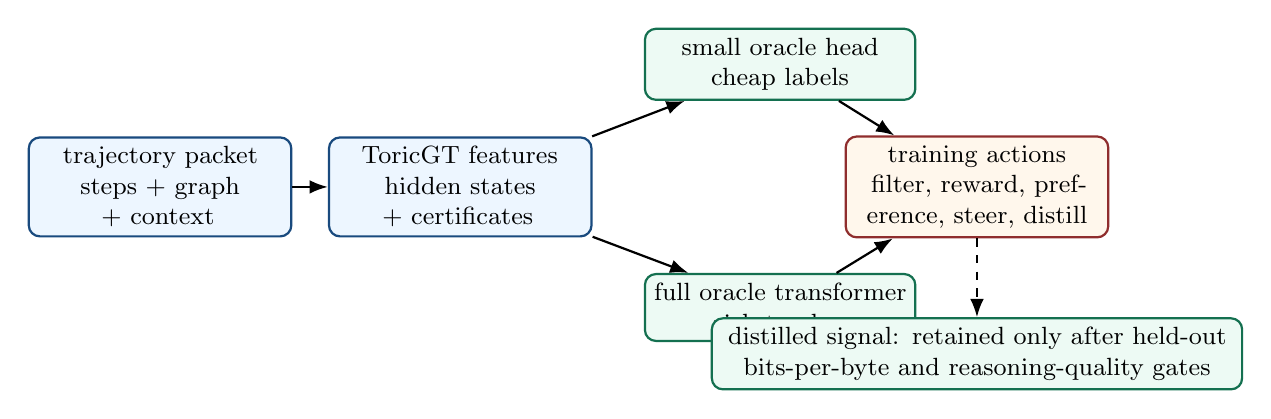
\begin{tikzpicture}[font=\small, node distance=0.55cm, >=Latex]
\tikzstyle{p}=[rounded corners, draw=darkblue, thick, fill=softblue, text width=3.1cm, minimum height=0.85cm, align=center]
\tikzstyle{q}=[rounded corners, draw=darkgreen, thick, fill=softgreen, text width=3.2cm, minimum height=0.85cm, align=center]
\tikzstyle{r}=[rounded corners, draw=darkred, thick, fill=softorange, text width=3.1cm, minimum height=0.85cm, align=center]
\node[p] (input) {trajectory packet\\steps + graph + context};
\node[p, right=0.45cm of input] (features) {ToricGT features\\hidden states + certificates};
\node[q, above right=0.45cm and 0.65cm of features] (head) {small oracle head\\cheap labels};
\node[q, below right=0.45cm and 0.65cm of features] (full) {full oracle transformer\\rich teacher};
\node[r, right=3.2cm of features] (actions) {training actions\\filter, reward, preference, steer, distill};
\draw[->, thick] (input) -- (features);
\draw[->, thick] (features) -- (head);
\draw[->, thick] (features) -- (full);
\draw[->, thick] (head) -- (actions);
\draw[->, thick] (full) -- (actions);
\node[q, below=1.0cm of actions, text width=6.5cm] (student) {distilled signal: retained only after held-out bits-per-byte and reasoning-quality gates};
\draw[->, thick, dashed] (actions) -- (student);
\end{tikzpicture}
\caption{Two oracle routes. A small head tests whether property labels are already encoded; a full oracle transformer supplies stronger offline supervision and reward signals.}
\label{fig:oracle-routes}
\end{figure}

\section{Mathematical foundations}
\subsection{Equivariance and invariance}
Trajectory labels should not depend on arbitrary graph ordering. Renumbering graph-of-thought vertices, MCP resource handles, or KG entity ids should relabel local judgments and preserve global judgments.

\begin{theorem}[Oracle equivariance]
Let $\Pi$ be a group of admissible relabelings of trajectory packet tokens. Suppose the trajectory tokenizer is equivariant, all attention masks are conjugated by token relabeling, all projections are shared over token types, and graph-level pooling is symmetric. Then the oracle transformer is equivariant for local labels and invariant for global labels.
\end{theorem}
\begin{proof}
The proof is by composition. Equivariant tokenization maps a relabeled packet to a permuted token table. Shared linear projections commute with row permutations. Masked softmax attention and tropical attention commute with simultaneous row/column permutation of their score matrices. Shared feed-forward layers, residuals, and layer normalizations are row-wise and therefore commute with token permutation. By induction over layers, hidden token states relabel equivariantly. Local decoders applied row-wise inherit equivariance. Global pooling by sum, mean, log-sum-exp, max, or invariant attention is symmetric, hence invariant.
\end{proof}

\subsection{Proper scoring and calibration}
\begin{theorem}[Cross-entropy identifies conditional property probabilities]
Let $Y_p\in\{0,1\}$ be a binary property and let $Z$ be the oracle input. Over all measurable predictors $q(Z)\in(0,1)$, the expected binary cross-entropy
\begin{equation}
\mathbb{E}\big[-Y_p\log q(Z)-(1-Y_p)\log(1-q(Z))\big]
\end{equation}
 is uniquely minimized almost surely by $q^\star(Z)=\mathbb{P}(Y_p=1\mid Z)$.
\end{theorem}
\begin{proof}
Condition on $Z=z$ and write $\eta=\mathbb{P}(Y_p=1\mid Z=z)$. The conditional risk is
\begin{equation}
R(q)=-\eta\log q-(1-\eta)\log(1-q).
\end{equation}
Differentiating gives $R'(q)=-\eta/q+(1-\eta)/(1-q)$, which vanishes exactly at $q=\eta$. The second derivative is positive on $(0,1)$, so this is the unique minimizer.
\end{proof}

This theorem matters because an oracle trained by proper scoring can be used as a calibrated control signal. A label ``unsafe tool path with probability $0.83$'' is more useful than a hard rejection without uncertainty.

\subsection{Bits-per-byte side-information theorem}
The oracle improves compression only if its signal predicts future bytes or helps the base model choose better trajectories. The basic information identity is the correct discipline.

\begin{theorem}[Oracle side information and bits-per-byte]
Let $B$ be the next byte or byte block, $C$ the strict prefix context, and $Z$ an oracle-visible trajectory property signal that is also prefix-measurable. Let $q_0(b\mid C)$ be the optimal predictor using $C$ and $q_1(b\mid C,Z)$ the optimal predictor using $(C,Z)$. Then the expected reduction in base-two log loss is
\begin{equation}
\mathbb{E}\big[-\log_2 q_0(B\mid C)+\log_2 q_1(B\mid C,Z)\big]=I(B;Z\mid C).
\end{equation}
For byte block length $L$, the expected bits-per-byte reduction is $I(B;Z\mid C)/L$ before artifact and compute costs.
\end{theorem}
\begin{proof}
The optimal log-loss predictor is the true conditional distribution. Thus the first expected loss is $H(B\mid C)$ and the second is $H(B\mid C,Z)$, both measured in bits. Their difference is $H(B\mid C)-H(B\mid C,Z)=I(B;Z\mid C)$. Dividing by $L$ gives the byte-normalized value.
\end{proof}

\begin{corollary}[Artifact-adjusted oracle utility]
If storing or computing an oracle code costs $A$ bits over an evaluation block of $L$ bytes, then a necessary condition for net compression utility is
\begin{equation}
I(B;Z\mid C) > A.
\end{equation}
More generally, an oracle component should be retained only when held-out bits-per-byte utility plus predeclared quality/control gains clears the deployment threshold.
\end{corollary}

\subsection{Property poset projection}
Oracle labels must obey entailments. Raw logits need not.

\begin{definition}[Isotonic property projection]
Given soft scores $s\in\RR^{\calP}$ and a property poset $(\calP,\preceq)$, the isotonic projection is
\begin{equation}
\Pi_{\preceq}(s)=\argmin_{z\in\RR^{\calP}}\sum_{p\in\calP}(z_p-s_p)^2
\quad\text{subject to}\quad p\preceq q\Rightarrow z_p\le z_q.
\end{equation}
\end{definition}

\begin{theorem}[Nonexpansiveness of property projection]
The isotonic projection $\Pi_{\preceq}$ is unique and nonexpansive in Euclidean norm:
\begin{equation}
\|\Pi_{\preceq}(s)-\Pi_{\preceq}(s')\|_2\le \|s-s'\|_2.
\end{equation}
\end{theorem}
\begin{proof}
The feasible set is a closed convex cone cut out by linear inequalities $z_p-z_q\le0$. Euclidean projection onto a nonempty closed convex set in a Hilbert space is unique and firmly nonexpansive. Applying that standard projection theorem gives the result.
\end{proof}

\subsection{Sheaf of local trajectory judgments}
A long trajectory is judged locally. Accuracy might fail in a citation block, tone might drift in a refusal branch, and tool discipline might fail at one MCP call. Local judgments must glue.

\begin{definition}[Behavior sheaf on a trajectory cover]
Let $\calU=\{U_i\}$ be a cover of trajectory vertices, context blocks, or time intervals. For each open set $U_i$, let $\calF(U_i)$ be a vector space of local property logits or calibrated probabilities. Restriction maps $\rho_{ij}:\calF(U_i)\to\calF(U_i\cap U_j)$ compare labels on overlaps. A family $(s_i)$ is a global behavior section when $\rho_{ij}s_i=\rho_{ji}s_j$ on every overlap.
\end{definition}

\begin{proposition}[Least-squares gluing bound]
Suppose each $\calF(U_i)$ is a finite-dimensional Hilbert space and restrictions are norm-nonincreasing. Let $\delta_{ij}=\|\rho_{ij}s_i-\rho_{ji}s_j\|$. The minimum Cech mismatch
\begin{equation}
\loss_{\mathrm{glue}}(s)=\sum_{i<j}\|\rho_{ij}s_i-\rho_{ji}s_j\|^2
\end{equation}
vanishes if and only if the local sections glue to a global section. If the associated Cech Laplacian has positive smallest nonzero eigenvalue $\lambda_1$, then the distance from $s=(s_i)$ to the space of global sections is at most $\lambda_1^{-1/2}\loss_{\mathrm{glue}}(s)^{1/2}$.
\end{proposition}
\begin{proof}
The Cech coboundary $d^0$ maps local sections to overlap disagreements. Its kernel is exactly the space of compatible local sections, i.e. global sections of the sheaf on the cover. The mismatch is $\|d^0s\|^2$. On the orthogonal complement of $\ker d^0$, the Cech Laplacian $(d^0)^\ast d^0$ has spectrum bounded below by $\lambda_1$, so $\|d^0s\|^2\ge \lambda_1\dist(s,\ker d^0)^2$.
\end{proof}

\subsection{Persistence stability for trajectory classification}
\begin{definition}[Persistence-aware oracle]
An oracle is persistence-Lipschitz if there are constants $L_H,L_D$ such that for trajectories $\tau,\tau'$,
\begin{equation}
\|O(\tau)-O(\tau')\|\le L_H\|H(\tau)-H(\tau')\|+L_D d_B(\mathrm{Dgm}(\calK_\tau),\mathrm{Dgm}(\calK_{\tau'})),
\end{equation}
where $d_B$ is bottleneck distance between persistence diagrams.
\end{definition}

\begin{proposition}[Robustness under filtration perturbation]
If a trajectory oracle is persistence-Lipschitz and the filtration functions of two trajectory complexes differ by at most $\eps$ in sup norm, then
\begin{equation}
\|O(\tau)-O(\tau')\|\le L_H\|H(\tau)-H(\tau')\|+L_D\eps.
\end{equation}
\end{proposition}
\begin{proof}
The standard stability theorem for persistent homology gives $d_B(\mathrm{Dgm}(\calK_\tau),\mathrm{Dgm}(\calK_{\tau'}))\le\eps$ when filtration functions differ by at most $\eps$. Substitute into the Lipschitz definition.
\end{proof}

\subsection{Toric chamber stability and quantization}
\begin{theorem}[Margin-preserving property quantization]
Let oracle logits be affine on a toric property chamber: $\ell_p(h)=\langle a_p,h\rangle+b_p$. Suppose quantized coefficients $(\hat a_p,\hat b_p)$ satisfy
\begin{equation}
\max_p\sup_{h\in K}|\ell_p(h)-\hat\ell_p(h)|\le\eps
\end{equation}
for a compact hidden-state set $K$. If a trajectory $h\in K$ has property fan margin $\Delta_{\calP}(h)>2\eps$, then quantization preserves the active property label.
\end{theorem}
\begin{proof}
Let $p^\star$ be the unique active label. For any $q\ne p^\star$,
\begin{equation}
\hat\ell_{p^\star}(h)-\hat\ell_q(h)\ge \ell_{p^\star}(h)-\ell_q(h)-2\eps\ge \Delta_{\calP}(h)-2\eps>0.
\end{equation}
Thus $p^\star$ remains uniquely active.
\end{proof}

\subsection{Oracle-guided policy improvement}
The oracle can guide training by assigning reward to trajectories, but it must not overpower task correctness.

\begin{definition}[Oracle-shaped reward]
Let $R_{\mathrm{task}}(\tau)$ be a verifier or human-preference reward and $u_\phi(\tau)$ an oracle desirability score derived from property probabilities. The shaped reward is
\begin{equation}
R_\phi(\tau)=R_{\mathrm{task}}(\tau)+\alpha u_\phi(\tau)-\beta c_{\mathrm{artifact}}(\tau)-\gamma c_{\mathrm{risk}}(\tau).
\end{equation}
\end{definition}

\begin{theorem}[KL-regularized oracle improvement]
Let $\pi_0(\tau\mid x)$ be a base trajectory policy and let $R_\phi$ be bounded. The unique maximizer of
\begin{equation}
\mathbb{E}_{\tau\sim\pi}[R_\phi(\tau)]-\eta\,\mathbb{E}_{x}\KL(\pi(\cdot\mid x)\|\pi_0(\cdot\mid x))
\end{equation}
over distributions absolutely continuous with respect to $\pi_0$ is
\begin{equation}
\pi_\phi(\tau\mid x)=\frac{\pi_0(\tau\mid x)\exp(R_\phi(\tau)/\eta)}{Z_\phi(x)}.
\end{equation}
The objective value is at least that of $\pi_0$.
\end{theorem}
\begin{proof}
For fixed $x$, the optimization is the Donsker-Varadhan variational formula. Completing the square in relative entropy gives
\begin{equation}
\mathbb{E}_\pi R_\phi-\eta\KL(\pi\|\pi_0)=\eta\log Z_\phi(x)-\eta\KL(\pi\|\pi_\phi),
\end{equation}
which is maximized uniquely by $\pi_\phi$. Choosing $\pi=\pi_0$ is feasible, so the maximum is at least the base value.
\end{proof}

\subsection{Ergodic oracle occupancy}
For deployed agents, we care about long-run behavior frequencies: how often the agent becomes overconfident, verbose, unsafe, or tool-inefficient.

\begin{theorem}[Oracle occupancy under stationary reasoning dynamics]
Let $(X_t)$ be an ergodic Markov chain on compact trajectory-step space with invariant distribution $\mu$. Let $g_p(X_t)$ be a bounded oracle score for property $p$. Then
\begin{equation}
\frac1T\sum_{t=0}^{T-1}g_p(X_t)\to \int g_p(x)\,d\mu(x)
\end{equation}
almost surely. The same holds for any bounded function of finitely many oracle properties, certificate residuals, and bits-per-byte-local losses.
\end{theorem}
\begin{proof}
This is the Markov-chain ergodic theorem for bounded measurable observables under ergodicity. The compactness assumption ensures no integrability issue for bounded oracle outputs.
\end{proof}

\section{Label construction and supervision sources}
\subsection{Label taxonomy}
ToricGT IV uses a typed label schema rather than a flat classifier. A minimal practical taxonomy is:
\begin{enumerate}
\item \textbf{Correctness:} correct, partially correct, unverifiable, contradiction, mathematical error, citation error, tool-output mismatch.
\item \textbf{Grounding:} grounded in retrieved evidence, unsupported but plausible, unsupported and false, memory-stale, KG-path unsupported, MCP-resource mismatch.
\item \textbf{Reasoning quality:} valid decomposition, invalid branch, coherent merge, circular proof, missing lemma, excessive search, unstable persistence, high derived residual.
\item \textbf{Behavior:} helpful, evasive, overconfident, sycophantic, emotionally mismatched, too terse, too verbose, domain-register mismatch.
\item \textbf{Compliance and safety:} follows user intent, asks needed clarification, refuses correctly, refuses unnecessarily, unsafe compliance, policy-boundary ambiguity.
\item \textbf{Efficiency:} good token economy, poor token economy, redundant retrieval, unnecessary tool call, insufficient tool use, high artifact cost, positive bits-per-byte utility.
\item \textbf{Memory/MCP discipline:} permission-respecting, stale-memory use, memory contamination, tool schema violation, resource provenance missing, prompt injection susceptibility.
\end{enumerate}

\subsection{Human labels, verifier labels, and weak labels}
No single label source is sufficient. Human labels capture tone, personality, refusal appropriateness, and nuanced compliance. Verifiers capture task success. Programmatic audits capture algebraic and graph consistency. Weak labels capture scale. The oracle should explicitly model source reliability.

\begin{definition}[Multi-source label model]
Let $Y_p$ be the latent true property and let $L_{p,s}$ be a label from source $s$ for property $p$. A multi-source label model has source confusion matrices
\begin{equation}
\Theta_{p,s}(a,b)=\mathbb{P}(L_{p,s}=b\mid Y_p=a),
\end{equation}
with priors tied by property family. Training alternates between estimating posterior soft labels $\mathbb{P}(Y_p\mid L_{p,1:S},\tau)$ and fitting the oracle to those soft labels.
\end{definition}

\subsection{Synthetic certificate labels}
Many labels can be generated exactly. For toric algebra tasks, compute toric ideals, Cox degrees, Hilbert bases, Cech residuals, Betti tables, and small resolutions offline. For graph tasks, compute shortest-path consistency, cut certificates, matching feasibility, proof-tree validity, and branch-merge compatibility. For behavior tasks, synthetic labels should be used carefully: they are useful for nonface constraints and tool-schema compliance but insufficient for human tone.

\subsection{Contrastive pairs}
ToricGT IV benefits from pairs of trajectories that solve the same task but differ in one property. Examples:
\begin{enumerate}
\item correct proof versus proof with one false lemma;
\item grounded answer versus hallucinated citation;
\item concise technical answer versus verbose but correct answer;
\item safe refusal with alternative versus unhelpful blanket refusal;
\item efficient two-call tool plan versus redundant ten-call plan;
\item coherent branch merge versus inconsistent branch merge;
\item current memory retrieval versus stale memory retrieval.
\end{enumerate}
Contrastive pairs train axes to be interpretable and reduce label superposition.

\section{Training objectives}
\subsection{Core supervised oracle objective}
Let $\hat y_p=O_\phi(\tau)_p$ be a probability, ordinal distribution, or continuous score. The core objective is
\begin{equation}
\loss_{\mathrm{sup}}=\sum_{p\in\calP}w_p\,\CE(y_p,\hat y_p),
\end{equation}
with label-source reliability weights and missing-label masks.

For ordinal labels $y_p\in\{0,\ldots,K_p\}$, use cumulative logits
\begin{equation}
\hat F_{p,k}(\tau)=\mathbb{P}(Y_p\le k\mid\tau)
\end{equation}
with monotonicity penalties $\max(0,\hat F_{p,k}-\hat F_{p,k+1})$.

\subsection{Structured oracle loss}
The structured loss combines property-poset, compatibility, calibration, sheaf, toric, and certificate terms:
\begin{align}
\loss_{\mathrm{oracle}}={}&\loss_{\mathrm{sup}}+\lambda_{\preceq}\loss_{\preceq}+\lambda_{\mathrm{SR}}\loss_{\mathrm{SR}}+\lambda_{\mathrm{cal}}\loss_{\mathrm{cal}}+\lambda_{\mathrm{glue}}\loss_{\mathrm{glue}}\\
&+\lambda_{\mathrm{fan}}\loss_{\mathrm{fan}}+\lambda_{\mathrm{pers}}\loss_{\mathrm{pers}}+\lambda_{\mathrm{der}}\loss_{\mathrm{der}}+\lambda_{\mathrm{ret}}\loss_{\mathrm{ret}}+\lambda_{\mathrm{eff}}\loss_{\mathrm{eff}}.
\end{align}
The components are:
\begin{align}
\loss_{\preceq}&=\sum_{p\preceq q}\max(0,\hat y_q-\hat y_p)^2,\\
\loss_{\mathrm{SR}}&=\sum_{F\in\mathrm{MinNonFaces}(\Delta)}w_F\prod_{p\in F}\hat y_p,\\
\loss_{\mathrm{cal}}&=\sum_{b\in\mathrm{bins}}\frac{|b|}{N}\left(\mathrm{conf}(b)-\mathrm{acc}(b)\right)^2,\\
\loss_{\mathrm{fan}}&=\mathbb{E}_\tau\max(0,\gamma-\Delta_{\calP}(\tau))^2,\\
\loss_{\mathrm{der}}&=\sum_t\|d_{t+1}f_t-f_{t-1}d_t\|_F^2,\\
\loss_{\mathrm{eff}}&=\max(0, c_{\mathrm{artifact}}-\widehat{\Delta \bitsperbyte}\cdot L)^2.
\end{align}
The loss is not always enabled. Use audit-only mode first; then probe-only; then adapter fine-tuning; then full-oracle teacher training; then base-model distillation.

\subsection{Trajectory contrastive objective}
For a pair $(\tau^+,
\tau^-)$ where $\tau^+$ is preferred for property $p$, use
\begin{equation}
\loss_{\mathrm{rank}}= -\log \sigma\left(s_p(\tau^+)-s_p(\tau^-)-m_p\right),
\end{equation}
where $m_p$ is a margin. For multi-property pairs, the margin is weighted by a signed property-difference vector.

\subsection{Oracle-to-base distillation}
The base model should not depend on a large oracle at inference unless ablations justify the cost. Distillation trains a small student signal:
\begin{equation}
\loss_{\mathrm{distill}}=\KL\bigl(O_\psi(\tau)\,\|\,O_{\mathrm{small}}(h_\theta(\tau))\bigr)+\lambda\|z_{\mathrm{small}}\|_0^{\mathrm{soft}}.
\end{equation}
The sparsity term encourages a compact code: a few property logits, margins, and warning flags rather than a full explanatory trace.

\section{Using the oracle to improve the model}
\subsection{Data selection and rejection sampling}
The simplest use is dataset filtering. Generate multiple candidate trajectories for a problem. Score them with the oracle. Keep trajectories that are correct, grounded, efficient, and behavior-compatible. Reject trajectories with high hallucination probability, unsafe-compliance risk, stale memory, or low verifier agreement. This improves supervised fine-tuning data without changing inference.

\subsection{Loss reweighting}
For a training token block $b_{1:L}$ generated by trajectory $\tau$, define a quality weight
\begin{equation}
w(\tau)=\exp\left(\alpha u_{\mathrm{quality}}(\tau)-\beta u_{\mathrm{risk}}(\tau)-\gamma u_{\mathrm{cost}}(\tau)\right).
\end{equation}
The weighted language-model loss is
\begin{equation}
\loss_{\mathrm{LM,w}}=\sum_t w(\tau_t)\bigl[-\log p_\theta(b_t\mid b_{<t})\bigr].
\end{equation}
Weights must be clipped to avoid destroying base distributional coverage.

\subsection{Preference optimization}
For two candidate outputs or trajectories $(\tau_a,
\tau_b)$, define oracle preference
\begin{equation}
\Delta_\phi = u_\phi(\tau_a)-u_\phi(\tau_b).
\end{equation}
Use it to construct preference pairs for DPO-style or reward-model training, but only after calibration checks show that the oracle agrees with held-out human/verifier judgments.

\subsection{GFlowNet and graph-of-thought reward shaping}
A graph-of-thought search policy can use terminal reward
\begin{equation}
R(\tau)=R_{\mathrm{task}}(\tau)\exp\left(\alpha u_{\mathrm{oracle}}(\tau)-\beta c_{\mathrm{risk}}(\tau)-\gamma c_{\mathrm{length}}(\tau)\right).
\end{equation}
This biases exploration toward trajectories that solve the task by desirable reasoning rather than by accidental final-answer matching.

\subsection{Retrieval and memory gates}
For a memory candidate $m$ and current trajectory prefix $\tau_{<t}$, retrieve by
\begin{equation}
S(q,m)=\langle Pq,Pm\rangle+\lambda_\Sigma\langle \Sigma(q),\Sigma(m)\rangle+\lambda_O\langle O(q),O(m)\rangle-\lambda_{\mathrm{bad}}r_{\mathrm{risk}}(m).
\end{equation}
The oracle term prevents retrieval of semantically similar but behaviorally incompatible memories, such as stale code snippets, unsafe tool traces, or overly verbose prior answers.

\subsection{MCP tool-call gating}
For each proposed MCP tool call, classify the local tool trajectory: schema compliance, permission safety, relevance, expected utility, and prompt-injection risk. Let $a$ be a proposed action. Execute only if
\begin{equation}
\mathbb{E}[U(a)\mid\tau]-\lambda_{\mathrm{risk}}\mathbb{P}(\mathrm{risk}\mid\tau,a)-\lambda_{\mathrm{cost}}c(a)>\kappa.
\end{equation}
This gives a principled link between the MCP substrate of ToricGT III and the behavior-classification objective of ToricGT IV.

\subsection{Test-time steering}
When the oracle is differentiable with respect to hidden states, it can define a local projection:
\begin{equation}
h^+=\argmin_{\tilde h}\frac12\|\tilde h-h\|_G^2+\lambda\,\dist(O_\phi(\tilde h),K_{\mathrm{desired}})^2+\eta\,\loss_{\mathrm{SR}}(O_\phi(\tilde h)).
\end{equation}
This should be used sparingly. In many cases the safer method is to train the base model with oracle-shaped examples rather than to steer at inference.

\section{Toric, sheaf, and representation-theoretic refinements}
\subsection{Cox-coordinate behavior codes}
Let $\Sigma$ be a behavior fan with one-dimensional cones $\rho\in\Sigma(1)$. A Cox-style behavior code uses variables $z_\rho$ for primitive behavior axes. A trajectory's soft code is $z_\rho(\tau)\in[0,1]$. The Cox degree records a behavior class:
\begin{equation}
\deg z^u = \sum_{\rho}u_\rho[D_\rho]\in \mathrm{Cl}(X_\Sigma).
\end{equation}
If a trajectory is intended to remain in a concise technical proof class, its Cox degree should be stable across local windows. Degree drift flags tone, verbosity, or proof-mode instability.

\subsection{Vector bundles of behavioral modes}
A full oracle can model behavior as a vector bundle over task/context space. The base point is the problem plus context state; the fiber contains allowed behavior coordinates. Local trivializations correspond to domains: math proof, coding, medical information, creative writing, refusal, summarization, retrieval, tool use.

\begin{definition}[Behavior vector bundle]
Let $X$ be a task-context space covered by charts $U_i$. A behavior vector bundle is local data $E_i=U_i\times\RR^r$ with transition functions $g_{ij}:U_i\cap U_j\to GL_r(\RR)$ satisfying $g_{ij}g_{jk}=g_{ik}$ on triple overlaps. An oracle section is a choice of behavior vector $s_i(x)\in E_i$ compatible on overlaps.
\end{definition}

The bundle view prevents a common failure: using one global personality axis for all domains. Warmth, uncertainty, compliance, and verbosity mean different things in mathematical proof, emergency safety, and creative brainstorming. Transitions let the oracle adapt while preserving a global section condition.

\subsection{Differential forms for drift and path dependence}
Let $\xi_t\in\RR^r$ be GraphCG behavior coordinates. A one-form $\omega=\sum_i f_i(\xi)d\xi_i$ measures local behavior work along a trajectory:
\begin{equation}
\int_\tau \omega = \sum_t \langle f(\xi_t),\xi_{t+1}-\xi_t\rangle.
\end{equation}
If $d\omega\approx0$, the accumulated score is approximately path-independent; if not, branch order matters. This is useful for detecting unstable tone or compliance dynamics across long reasoning paths.

\subsection{Young tableaux and representation-theoretic labels}
Some trajectory types are combinatorial. A proof may decompose into lemmas with dependencies; a tool plan may have interleaving resource constraints; a long answer may require ordered slots. Young tableaux provide finite normal forms for such structured labels.

\begin{example}[Tableau label for proof obligations]
Let a proof trajectory have obligations grouped by type: definitions, lemmas, computations, citations, and verifier checks. Encode the order in a semistandard tableau whose rows represent compatible parallel obligations and columns represent strict dependency. The oracle predicts the tableau shape $\lambda$, filling content, and violation count. A bad merge often appears as a column violation or a Littlewood-Richardson coefficient mismatch when combining two branches.
\end{example}

Representation-theoretic labels are optional. They are most useful when a domain has genuine symmetry: root-system tasks, algebraic proof tasks, program transformations, morphology, symbolic tableaux, or structured multimodal layout. The rule remains pragmatic: use them only if they improve task quality or compression.

\section{Oracle training schedule}
\subsection{Stage 0: audit-only}
Run the base model and collect trajectory packets. Compute oracle features without training: verifier scores, property weak labels, certificate residuals, sheaf-gluing errors, retrieval quality, memory hygiene, tool-call outcomes, tone metrics, and bits-per-byte slices. This establishes label reliability and class balance.

\subsection{Stage 1: frozen head}
Freeze the base model. Train a linear or shallow oracle head on pooled hidden states and certificate summaries. Report per-property AUROC, calibration error, class-balanced F1, false-negative rate for high-risk properties, and mutual information with future bytes. Poor frozen-head performance indicates missing representation or poor labels.

\subsection{Stage 2: adapter oracle}
Unfreeze small adapters and train the head with small weights. Maintain the base language loss. Use ratio caps so auxiliary gradients cannot dominate next-token training:
\begin{equation}
\frac{\|\nabla\loss_{\mathrm{oracle}}\|}{\|\nabla\loss_{\mathrm{LM}}\|+\eps}\le r_{\max}.
\end{equation}

\subsection{Stage 3: full oracle transformer}
Train $\Omega_\psi$ offline on full trajectory packets. Use it for filtering, preference labels, reward shaping, and teacher distillation. Do not deploy it unless inference-time oracle classification is a product requirement and ablations justify latency and artifact cost.

\subsection{Stage 4: distillation and promotion}
Distill the full oracle to a small head or quantized code. Promote only if:
\begin{enumerate}
\item held-out bits-per-byte improves or remains within tolerance while a predeclared reasoning/control metric improves;
\item high-risk false negatives decrease;
\item calibration remains stable out of domain;
\item artifact bytes and latency are acceptable;
\item no data-leakage or score-before-update violation is introduced.
\end{enumerate}

\section{Implementation blueprint}
\subsection{Trajectory record schema}
\begin{lstlisting}[language=Python]
@dataclass
class TrajectoryPacket:
    task_id: str
    prefix_hash: str
    step_nodes: Tensor          # [T, N, d]
    graph_edges: LongTensor     # graph-of-thought, retrieval, MCP, memory edges
    output_tokens: LongTensor
    verifier_scores: Tensor
    evidence_spans: list[EvidenceSpan]
    mcp_events: list[MCPEvent]
    memory_refs: list[MemoryRef]
    kg_paths: list[KGPath]
    filtered_complex: ComplexSummary
    persistence: PersistenceSummary
    derived_residuals: Tensor
    sheaf_gluing: Tensor
    toric_chart: ToricChartCode
    behavior_coordinates: Tensor
    labels: dict[str, LabelValue]
    label_sources: dict[str, list[str]]
\end{lstlisting}

\subsection{Oracle head interface}
\begin{lstlisting}[language=Python]
class OracleHead(nn.Module):
    def forward(self, hidden_summary, cert_summary, context_summary):
        z = torch.cat([hidden_summary, cert_summary, context_summary], dim=-1)
        logits = self.property_logits(z)
        ordinal = self.ordinal_heads(z)
        margins = self.fan_margin_head(z)
        return OracleOutput(logits=logits, ordinal=ordinal, margins=margins)
\end{lstlisting}

\subsection{Full oracle transformer interface}
\begin{lstlisting}[language=Python]
class OracleTransformer(nn.Module):
    def forward(self, packet_tokens, graph_edges, masks):
        z = self.token_embed(packet_tokens)
        z = self.graph_tropical_blocks(z, graph_edges, masks)
        pooled = invariant_pool(z, masks)
        local = self.local_property_decoder(z)
        global_out = self.global_property_decoder(pooled)
        return local, global_out
\end{lstlisting}

\subsection{Minimal training loop}
\begin{lstlisting}[language=Python]
for batch in loader:
    with torch.no_grad() if freeze_base else contextlib.nullcontext():
        base_out = base_model(batch.inputs, return_trajectory=True)
    packet = build_packet(batch, base_out)
    oracle_out = oracle(packet)
    loss = supervised_loss(oracle_out, packet.labels)
    loss += lambda_poset * poset_loss(oracle_out)
    loss += lambda_sr * stanley_reisner_loss(oracle_out)
    loss += lambda_glue * sheaf_gluing_loss(oracle_out, packet.cover)
    loss += lambda_cal * calibration_loss(oracle_out, packet.labels)
    loss.backward()
    optimizer.step()
\end{lstlisting}

\section{Evaluation and ablations}
\subsection{Oracle metrics}
Report, per property and per slice:
\begin{enumerate}
\item AUROC, AUPRC, class-balanced F1, false-positive and false-negative rates;
\item expected calibration error and reliability plots;
\item poset violation mass and Stanley-Reisner nonface mass;
\item local-to-global gluing error;
\item fan-margin distribution and quantization stability;
\item trajectory-level agreement with human labels and verifier labels;
\item out-of-domain degradation.
\end{enumerate}

\subsection{Model-improvement metrics}
The oracle is justified only by downstream effects:
\begin{enumerate}
\item held-out bits-per-byte globally and on reasoning-heavy slices;
\item verified task success and mathematical/procedural accuracy;
\item reduction in hallucinated citations and unsupported claims;
\item fewer unsafe-compliance and unnecessary-refusal cases;
\item improved retrieval precision and stale-memory rejection;
\item reduced redundant tool calls and lower context budget for same quality;
\item tone/personality corridor stability under long-context and multi-turn settings.
\end{enumerate}

\subsection{Ablation protocol}
Ablate in this order:
\begin{enumerate}
\item remove oracle entirely;
\item frozen head only;
\item adapter head;
\item full oracle as data filter only;
\item full oracle as preference teacher;
\item full oracle as GFlowNet reward;
\item inference-time steering;
\item each structured loss: poset, Stanley-Reisner, sheaf gluing, toric fan, persistence, derived, calibration.
\end{enumerate}
Every ablation must report artifact bytes, latency, bits-per-byte, verifier success, high-risk false negatives, and calibration.

\section{Catalogue of ToricGT IV oracle objectives}
The following objectives are intended as a concrete menu. Use audit-only first; train only after label reliability is acceptable; deploy only after ablation.

\subsection{Classifier and calibration objectives}
\begin{enumerate}
\item \textbf{Trajectory property cross-entropy.} Multi-label CE over atomic properties. Helps by making hidden reasoning states linearly legible for accuracy, tone, compliance, and efficiency.
\item \textbf{Ordinal severity loss.} Cumulative-link loss for severity labels: harmless issue, minor issue, major issue, catastrophic issue. Useful for safety and hallucination triage.
\item \textbf{Calibration energy.} Differentiable expected calibration error plus Brier score. Prevents overconfident steering and improves threshold reliability.
\item \textbf{Abstention/selective-risk loss.} The oracle may output ``uncertain''. Train coverage-risk curves so the system knows when not to trust the classifier.
\item \textbf{Property fan margin.} Encourage large margins between incompatible behavior chambers. Useful for quantized deployment and stable control.
\end{enumerate}

\subsection{Algebraic and topological objectives}
\begin{enumerate}[resume]
\item \textbf{Property poset monotonicity.} Penalize entailment violations. Makes labels compositional: severe hallucination implies unsupported claim.
\item \textbf{Stanley-Reisner compatibility.} Penalize forbidden coactivations, such as high confidence and no evidence.
\item \textbf{Cech gluing loss.} Ensure local window judgments agree on overlaps. Detects local tone or evidence inconsistencies.
\item \textbf{Persistence stability loss.} Pair nearby trajectories and penalize large label changes when persistence diagrams are close.
\item \textbf{Derived residual classification.} Use mapping-cone residuals to classify branch-merge failures and invalid analogies.
\item \textbf{Cox-degree behavior drift.} Penalize unexplained changes in behavior class degree across trajectory windows.
\item \textbf{Differential-form path-dependence loss.} Penalize large $d\omega$ when behavior score should be path-independent.
\item \textbf{Vector-bundle transition loss.} Train domain-specific tone/personality transitions satisfying cocycle consistency.
\item \textbf{Tableau normal-form loss.} Classify proof or plan structures by Young-tableau shapes and penalize invalid fillings.
\item \textbf{Root-system chamber loss.} For symmetric tasks, classify Weyl chamber transitions and penalize invalid crossings.
\end{enumerate}

\subsection{Training-control objectives}
\begin{enumerate}[resume]
\item \textbf{Oracle-weighted SFT.} Weight supervised tokens by oracle quality, clipped for stability.
\item \textbf{Oracle preference distillation.} Turn trajectory pairs into preference data for DPO or reward training.
\item \textbf{GFlowNet desirability reward.} Shape graph-of-thought search toward accurate, grounded, behavior-compatible trajectories.
\item \textbf{Retrieval compatibility loss.} Train memory retrieval to prefer oracle-compatible helper trajectories.
\item \textbf{MCP tool discipline loss.} Classify and penalize irrelevant, unsafe, schema-invalid, or redundant tool calls.
\item \textbf{Context economy objective.} Predict marginal utility of adding each context block; train the model to stop context filling when utility falls below cost.
\item \textbf{Bits-per-byte utility head.} Predict whether an oracle code or retrieved block improves held-out bits-per-byte after artifact cost.
\item \textbf{High-risk false-negative penalty.} Asymmetrically penalize missed unsafe compliance, hallucination, and privacy/memory leakage.
\item \textbf{Persona corridor stability.} Penalize unwarranted tone/personality drift across multi-turn or long-context trajectories.
\item \textbf{Verifier disagreement triage.} Classify cases where oracle confidence conflicts with verifier output and trigger abstention or additional evidence retrieval.
\end{enumerate}

\section{Pragmatic deployment rules}
\subsection{When to deploy a head}
Deploy a small oracle head only if it satisfies all of the following:
\begin{enumerate}
\item high-risk properties are calibrated and false negatives are below threshold;
\item output decisions are stable under quantization and prompt paraphrase;
\item head latency is acceptable;
\item held-out bits-per-byte does not regress unless a predeclared safety/control metric improves enough to justify the cost;
\item the head does not create a future-token leakage channel;
\item the head improves at least one training or inference decision in ablation.
\end{enumerate}

\subsection{When to keep it teacher-side}
Keep the oracle teacher-side when it improves data filtering, reward labeling, or checkpoint selection but is too expensive, too brittle, too poorly calibrated, or not useful for live inference. Most full oracle transformers will be teacher-side.

\subsection{Failure modes}
\begin{enumerate}
\item \textbf{Aesthetic overfitting:} the oracle rewards polished tone but not correctness.
\item \textbf{Sycophancy amplification:} helpfulness labels confuse agreement with usefulness.
\item \textbf{Verifier monoculture:} the oracle learns one verifier's blind spots.
\item \textbf{Label leakage:} trajectory labels accidentally encode future validation bytes.
\item \textbf{Over-steering:} inference projections degrade creativity or domain adaptation.
\item \textbf{Unsafe confidence:} calibrated properties become uncalibrated after distribution shift.
\item \textbf{Memory contamination:} oracle-compatible memories reinforce a previous wrong belief.
\end{enumerate}


\section{Capacity theory for oracle heads and full oracle transformers}
\subsection{When a head is enough}
A central engineering question is whether the classifier should be a small head or a full oracle model. The answer depends on sufficiency of the base hidden representation.

\begin{definition}[Property-sufficient representation]
Let $Z_\theta(\tau)$ be a hidden representation of a trajectory packet. It is property-sufficient for labels $Y_\calP$ if
\begin{equation}
\mathbb{P}(Y_\calP\mid \tau)=\mathbb{P}(Y_\calP\mid Z_\theta(\tau))
\end{equation}
almost surely.
\end{definition}

\begin{proposition}[Frozen-head optimality under sufficiency]
If $Z_\theta$ is property-sufficient and the head class contains all conditional distributions on $Y_\calP$ as functions of $Z_\theta$, then the optimal head attains the Bayes risk of any oracle that reads the full trajectory.
\end{proposition}
\begin{proof}
By sufficiency, the conditional law of $Y_\calP$ given the full packet equals the conditional law given $Z_\theta$. Proper scoring is minimized by the true conditional law. Since the head class contains that law, it attains the full-packet Bayes risk.
\end{proof}

This proposition is practical: train a frozen head first. If it nearly matches a full oracle on held-out labels, the full oracle is unnecessary for deployment. If it fails specifically on tool discipline, memory freshness, or citation grounding, the base hidden state lacks those features and should be augmented or trained.

\subsection{When a full oracle is necessary}
The head is insufficient when property labels depend on information absent from hidden summaries: exact tool schemas, raw evidence spans, graph paths, permission boundaries, or long-context block provenance. A full oracle can recover such information by reading the trajectory packet directly.

\begin{theorem}[Bounded-packet universal oracle approximation]
Fix maximum packet size, finite type vocabularies, bounded real fields, and admissible graph relabelings. Let $f:\calT\to\RR^m$ be a continuous graph-invariant global property map and $g:\calT\to\RR^{N\times r}$ a continuous graph-equivariant local property map. A graph-token oracle transformer with equivariant tokenization, shared attention, shared feed-forward layers, and symmetric pooling can uniformly approximate $(f,g)$ on the bounded packet space.
\end{theorem}
\begin{proof}
The bounded packet space is a finite union of compact cells indexed by masks, graph incidence, and type patterns. On each cell, a continuous equivariant map can be conjugated through an injective equivariant tokenizer to a continuous equivariant sequence map on a compact token domain. Transformer universality for bounded sequences with shared token operations gives uniform approximation on each cell. A finite discrete selector over cells combines the approximants. Symmetric pooling gives invariant outputs, and row-wise local decoders give equivariant outputs.
\end{proof}

The theorem is not a claim that a finite oracle solves arbitrary-length reasoning. It says that, for the bounded packet domain used in training and validation, a full oracle transformer is expressive enough to learn the desired continuous property map if data and optimization permit.

\section{A multigraded algebra of trajectory labels}
\subsection{Label rings}
The property set has algebraic structure. Let $S_\calP=k[z_p:p\in\calP]$ and assign each variable a multidegree
\begin{equation}
\deg z_p=(d_{\mathrm{task}},d_{\mathrm{evidence}},d_{\mathrm{behavior}},d_{\mathrm{safety}},d_{\mathrm{cost}})\in\ZZ^5.
\end{equation}
The quotient
\begin{equation}
R_\Delta=S_\calP/I_\Delta
\end{equation}
removes incompatible coactivations. A trajectory label distribution becomes a point in a soft version of $\Spec R_\Delta$. Multigrading makes it possible to ask whether the oracle is confusing evidence properties with tone properties, or cost properties with safety properties.

\begin{definition}[Multigraded property module]
A multigraded property module is a finitely generated $R_\Delta$-module $M=\oplus_{a\in\ZZ^k}M_a$ whose graded pieces encode label families at different scopes: token, step, branch, final answer, memory event, tool event, and whole trajectory.
\end{definition}

A free resolution
\begin{equation}
\cdots\to F_2\to F_1\to F_0\to M\to 0
\end{equation}
encodes relations among labels. For instance, a relation might say that ``safe refusal with no alternative'' and ``user request answerable safely'' imply an unhelpfulness warning. Syzygies among such relations capture higher-order conflicts.

\subsection{Resolution-guided oracle regularization}
Let $\widehat d_i(\tau)$ be oracle-predicted differentials between soft free modules. Define
\begin{equation}
\loss_{\mathrm{label\mbox{-}res}}=\sum_i\|\widehat d_i(\tau)\widehat d_{i+1}(\tau)\|_F^2+\beta\sum_{i,a}|\widehat\beta_{i,a}(\tau)-\beta_{i,a}^{\star}|^2.
\end{equation}
This is useful when label conflicts are compositional. A model that learns only independent labels can still emit impossible combinations. A resolution-aware oracle learns the relations.

\begin{proposition}[Resolution loss detects first-order incompatibility]
Suppose $F_1\to F_0\to M$ presents a property module and a predicted label vector violates a defining relation represented by a row of $d_1$. Then the corresponding component of $\widehat d_1\hat z$ is nonzero. If all first-order relations are represented in $d_1$, then $\widehat d_1\hat z=0$ is exactly the linearized compatibility condition.
\end{proposition}
\begin{proof}
A presentation identifies $M$ with $F_0/\im d_1$. A vector in $F_0$ descends to a compatible module element exactly modulo the submodule of relations. Evaluating the relation rows on the soft vector gives zero precisely when the vector satisfies the represented linearized relations.
\end{proof}

\section{Oracle control as a closed-loop system}
\subsection{Controlled dynamics}
Let $x_t$ be a reasoning state, $a_t$ a model action such as next-token block, tool call, retrieval expansion, memory write, or branch merge, and $o_t=O_\phi(x_{0:t},a_t)$ the oracle property vector. A controlled ToricGT process has transition kernel
\begin{equation}
P_\theta(dx_{t+1}\mid x_t,a_t,r_t),
\end{equation}
where $r_t$ may include retrieved memory, MCP tool output, and verifier feedback.

\begin{definition}[Desirable invariant set]
A set $K\subset\calX$ is a desirable invariant set if states in $K$ satisfy required bounds on accuracy risk, unsafe-compliance probability, tone/personality corridor distance, evidence support, and context cost. It is $\delta$-invariant under policy $\pi$ if
\begin{equation}
\mathbb{P}_\pi(x_{t+1}\notin K\mid x_t\in K)\le\delta.
\end{equation}
\end{definition}

\begin{theorem}[One-step risk gate]
Suppose an oracle risk score $r(x,a)$ is calibrated, and action $a$ is allowed only when $r(x,a)\le \alpha$. If the event $x_{t+1}\notin K$ is contained in the calibrated risk event, then the gated policy is $\alpha$-invariant.
\end{theorem}
\begin{proof}
For $x_t\in K$, the gate ensures $\mathbb{P}(\mathrm{risk}\mid x_t,a_t)\le\alpha$. Since leaving $K$ implies the risk event by assumption, $\mathbb{P}(x_{t+1}\notin K\mid x_t,a_t)\le\alpha$. Taking expectation over allowed actions preserves the bound.
\end{proof}

\subsection{Stability versus capability}
There is a tension: strong oracle gates increase reliability but may reduce capability by blocking exploratory trajectories. ToricGT IV therefore uses three levels of action:
\begin{enumerate}
\item \textbf{Train-time shaping:} preferred default; improves the policy before deployment.
\item \textbf{Soft inference warning:} attach additional verification or retrieval when oracle risk is high.
\item \textbf{Hard gate:} reserved for high-stakes or policy-critical actions such as unsafe tool use or memory writes.
\end{enumerate}

\section{Long-context oracle classification}
\subsection{Context-window trajectory types}
In ToricGT III, the context window is a large canvas with length $L_C\le 10^7$ filled by retrieved memory, MCP resource text, KG neighborhoods, tool outputs, scratch reasoning blocks, verifier traces, and final answer sections. ToricGT IV classifies the fill policy itself. The oracle asks whether each block has positive marginal utility, whether evidence is duplicated, whether memory is stale, whether tool returns are used correctly, and whether the final answer depends on unsupported blocks.

\begin{definition}[Marginal context utility label]
For a context block $c_j$ inserted into prefix $C$, define its empirical marginal utility as
\begin{equation}
U_j=\Delta \mathrm{Score}(C,c_j)-\lambda_{\mathrm{tok}}|c_j|-\lambda_{\mathrm{lat}}\mathrm{latency}(c_j)-\lambda_{\mathrm{risk}}\mathrm{risk}(c_j),
\end{equation}
where $\Delta\mathrm{Score}$ can be verifier improvement, held-out bits-per-byte lift on a development set, retrieval recall gain, or task success improvement. The oracle label is positive when $U_j>0$.
\end{definition}

\subsection{Tropical ring attention as oracle evidence}
Tropical ring attention exposes active predecessors and margins over long contexts. The oracle should use active evidence paths rather than all tokens uniformly. For a query block $q$ and candidate evidence blocks $e_j$, define
\begin{equation}
A(q)=\argmax_j \{s(q,e_j)+v(e_j)\}.
\end{equation}
An answer is well grounded only if claims in the answer can be matched to active evidence blocks with stable margins. The oracle can classify low-margin claims as fragile even if the final answer appears correct.

\section{Detailed use cases}
\subsection{Mathematical proof trajectories}
A proof trajectory contains definitions, lemmas, computations, branch attempts, and final synthesis. The oracle labels missing hypotheses, invalid lemma use, circular dependency, proof gap, theorem mismatch, and overconfident final wording. Toric features enter through proof obligation complexes: definitions and lemmas are vertices, dependencies are edges, completed subproofs are higher faces, and invalid merges create boundary residuals.

\subsection{Coding-agent trajectories}
A coding trajectory contains repository retrieval, file edits, test runs, error traces, and patch explanations. The oracle labels whether the model used relevant files, respected constraints, ran adequate tests, avoided spurious edits, and summarized changes accurately. MCP tool-call gating is particularly useful here: classify tool schema validity and whether the next call is necessary.

\subsection{Knowledge-graph question answering}
A KG trajectory contains entity linking, neighborhood expansion, path selection, evidence synthesis, and answer generation. The oracle labels path relevance, unsupported relation jumps, stale KG edges, citation mismatch, and path redundancy. Toric property chambers separate ``enough evidence'', ``needs disambiguation'', and ``unsupported answer''.

\subsection{Markdown memory and persona stability}
A markdown memory trajectory contains read, select, update, and write operations over memory blocks. The oracle labels whether a memory is relevant, stale, user-specific, privacy-sensitive, or behaviorally contaminating. Personality control is handled as a bundle: the same style vector has different permitted intervals depending on task chart.

\subsection{Safety and refusal trajectories}
A safety trajectory contains intent classification, policy-boundary reasoning, allowed-content extraction, refusal text, and safe alternative. The oracle labels unnecessary refusal, unsafe compliance, missing safe alternative, excessive moralizing, and tone mismatch. Stanley-Reisner nonfaces prevent incompatible labels such as ``unsafe compliance'' and ``safe refusal'' from both being high.

\subsection{Scientific literature synthesis}
A literature trajectory contains retrieval, relevance screening, claim extraction, contradiction tracking, and final synthesis. The oracle labels citation support, overgeneralization, uncertainty quality, and whether the output distinguishes evidence from speculation. Differential-form path-dependence can flag cases where conclusion changes depending on evidence order.

\subsection{Long-context summarization}
A summarization trajectory fills a large context with sections and decides what to keep. The oracle labels coverage, redundancy, hallucinated compression, omission of critical caveats, and context economy. Marginal context utility labels train the model to stop adding low-value blocks.

\subsection{Tool-augmented data analysis}
A data-analysis trajectory contains table loading, transformation, plotting, statistical testing, and final interpretation. The oracle labels schema mismatch, invalid aggregation, overclaiming, missing uncertainty, and plot-text inconsistency.

\subsection{Multi-agent debate and verifier loops}
A debate trajectory contains multiple candidate solutions, critiques, verifier checks, and final aggregation. The oracle labels whether critique actually addresses evidence, whether final aggregation resolves contradictions, and whether one branch dominates without justification.

\subsection{Behavior-preserving translation or rewriting}
A rewriting trajectory must preserve meaning while changing tone, register, or language. The oracle labels semantic drift, tone success, personality compatibility, and unnecessary content insertion. Representation-theoretic normal forms can help when transformations have compositional structure.

\section{Extended catalogue of oracle-derived objectives}
\subsection{Data and label objectives}
\begin{enumerate}[resume]
\item \textbf{Multi-source denoising objective.} Estimate source reliability and train on posterior soft labels rather than raw labels.
\item \textbf{Counterfactual edit objective.} Edit one property of a trajectory while preserving all others; penalize unintended label changes.
\item \textbf{Slice-balanced property loss.} Equalize performance across math, coding, safety, retrieval, and natural prose slices.
\item \textbf{Adversarial label stress test.} Generate near-boundary trajectories and require calibrated uncertainty.
\item \textbf{Human-oracle disagreement mining.} Sample high-disagreement cases for human review.
\end{enumerate}

\subsection{Control and deployment objectives}
\begin{enumerate}[resume]
\item \textbf{Safe-action threshold loss.} Optimize calibrated thresholds for MCP calls, memory writes, and high-risk answers.
\item \textbf{Oracle-triggered retrieval loss.} When the oracle predicts low grounding, train the agent to retrieve more evidence rather than hallucinate.
\item \textbf{Oracle-triggered clarification loss.} When intent ambiguity is high, train the model to ask a concise clarifying question.
\item \textbf{Tone repair objective.} Generate minimal edits that move a response into the tone corridor without changing factual content.
\item \textbf{Memory quarantine objective.} Learn to mark memories that are stale, untrusted, or behaviorally contaminating.
\item \textbf{Tool-call economy objective.} Penalize tool calls whose oracle-predicted marginal utility is below cost.
\item \textbf{Verifier escalation objective.} Trigger external verification when oracle confidence and task risk cross a threshold.
\item \textbf{Long-context pruning objective.} Drop context blocks with negative predicted marginal utility.
\item \textbf{Oracle consistency under paraphrase.} Require stable labels under input paraphrases and graph isomorphisms.
\item \textbf{Quantized-head stability objective.} Train logits so int8 or low-rank quantization preserves property chambers.
\end{enumerate}

\subsection{Geometric and algebraic objectives}
\begin{enumerate}[resume]
\item \textbf{Property polytope occupancy entropy.} Avoid collapse to one behavior chamber except where appropriate.
\item \textbf{One-dimensional-cone axis sparsity.} Encourage sparse use of primitive behavior axes for interpretability.
\item \textbf{Cech disagreement localization.} Attribute global label failure to the smallest local window causing overlap mismatch.
\item \textbf{Vector-bundle cocycle audit.} Ensure behavior-coordinate transitions compose consistently across task charts.
\item \textbf{Derived cone failure classifier.} Predict whether a branch merge fails because of missing evidence, conflicting assumptions, or invalid transformation.
\item \textbf{Tableau branch-order loss.} Penalize proof or plan branch order that violates semistandard constraints.
\item \textbf{Weyl-chamber symmetry loss.} Require symmetric tasks to receive labels transformed by the corresponding group action.
\item \textbf{Ergodic behavior budget loss.} Penalize long-run frequency of undesirable trajectory types above a bound.
\item \textbf{Oracle mutual-information estimator.} Estimate $I(B;Z\mid C)$ for oracle codes and prune low-utility codes.
\item \textbf{Artifact-aware Pareto objective.} Optimize quality, risk, latency, artifact bytes, and bits-per-byte as a Pareto frontier rather than a single scalar.
\end{enumerate}

\section{A complete ToricGT IV training recipe}
\subsection{Recommended default}
The default recipe is deliberately conservative.
\begin{enumerate}
\item Collect trajectories from the base model, including failed and low-quality samples.
\item Compute finite ToricGT certificates and ordinary verifier metrics.
\item Create a small property taxonomy with no more than $20$ initial labels.
\item Train a frozen oracle head and audit calibration.
\item Use the oracle only for data selection and trajectory rejection.
\item Train a base-model ablation on the filtered data.
\item If verified quality improves without bits-per-byte regression, add preference pairs.
\item If preference training succeeds, train a full oracle teacher for difficult labels.
\item Distill only the useful subset back into a compact head.
\end{enumerate}

\subsection{Escalation path}
Escalate to a full oracle transformer only when at least one of the following holds: the head misses labels requiring raw evidence spans; graph-of-thought topology matters; long-context block attribution matters; MCP tool schemas matter; or local-to-global behavior gluing cannot be recovered from pooled hidden states.

\section{Limits and safety considerations}
\subsection{Oracle labels are not ground truth}
An oracle can be wrong, biased, overfit, or miscalibrated. Its outputs should be treated as probabilistic training signals. For high-stakes actions, oracle labels should trigger additional verification rather than automatic suppression or compliance.

\subsection{Do not optimize personality at the expense of truth}
Tone and personality are secondary to factuality, safety, and user intent. The objective weights should reflect this. A polite hallucination is worse than a terse correct answer when accuracy is central.

\subsection{Avoid hidden chain exposure}
The oracle can operate on hidden summaries, graph certificates, and local labels without exposing private reasoning text. Training should not require showing full hidden chain-of-thought to users. Instead, expose concise rationales, citations, verifier status, and uncertainty when appropriate.


\section{Discussion}
ToricGT IV reframes behavior control as trajectory typing. This is stricter than final-answer classification and more pragmatic than unconstrained interpretability. The oracle does not need to expose private chain-of-thought text; it can classify finite trajectory packets, hidden summaries, graph structure, evidence events, and certificate residuals. The mathematical role of toric geometry, sheaves, persistence, representation theory, and ergodic dynamics is to make those labels structured, compositional, auditable, and compact.

The most important engineering distinction is between \emph{oracle accuracy} and \emph{oracle utility}. A full oracle transformer might classify trajectories beautifully and still be useless for deployment if it adds latency, artifact bytes, or false security. Conversely, a small head with only ten well-calibrated properties may produce substantial gains if it filters bad training data, improves GFlowNet search, rejects stale memory, or catches high-risk false negatives. The research program should therefore report both scientific oracle metrics and downstream model-improvement metrics.

\section{Conclusion}
ToricGT IV completes a natural arc. ToricGT I supplies finite algebraic certificates for graph-token reasoning. ToricGT II studies their dynamics through persistence, sheaves, vector bundles, differential forms, derived objects, and ergodic summaries. ToricGT III moves them into external context systems: MCPs, markdown memory, knowledge graphs, vector retrieval, quantization, and long-context tropical ring attention. ToricGT IV trains an oracle to classify the resulting trajectories by properties that matter: accuracy, reasoning quality, compliance, safety, tone, personality, efficiency, retrieval discipline, memory hygiene, and bits-per-byte utility.

The oracle is useful when it changes training decisions. It can select better data, shape graph-of-thought search, train preferences, control retrieval, gate MCP calls, prevent stale-memory use, improve calibration, and distill compact control signals into the base model. Its mathematical structure is not optional ornamentation; it is what makes the classifier compositional and auditable. But the final criterion remains empirical and severe: retain only the pieces that improve held-out bits-per-byte, verified reasoning, behavior reliability, or artifact efficiency.

\appendix
\section{Additional proof details}
\subsection{Stanley-Reisner gradients}
For a minimal nonface $F$, the penalty $\prod_{p\in F}\hat y_p$ has gradient
\begin{equation}
\frac{\partial}{\partial \hat y_q}\prod_{p\in F}\hat y_p=
\begin{cases}
\prod_{p\in F\setminus\{q\}}\hat y_p,& q\in F,\\
0,& q\notin F.
\end{cases}
\end{equation}
Thus the penalty concentrates on jointly high forbidden activations and is small when at least one incompatible property is confidently low.

\subsection{A conservative threshold rule}
Let $p_{\mathrm{risk}}(\tau)$ be a calibrated risk probability and $C_{\mathrm{FN}},C_{\mathrm{FP}}$ be false-negative and false-positive costs. The Bayes action is to block or escalate when
\begin{equation}
p_{\mathrm{risk}}(\tau)C_{\mathrm{FN}}>(1-p_{\mathrm{risk}}(\tau))C_{\mathrm{FP}}.
\end{equation}
Equivalently, block when $p_{\mathrm{risk}}(\tau)>C_{\mathrm{FP}}/(C_{\mathrm{FN}}+C_{\mathrm{FP}})$. This is why calibration is not cosmetic: it directly determines threshold correctness.

\section{Recommended initial experiment}
A minimal ToricGT IV experiment should avoid the full oracle at first.
\begin{enumerate}
\item Generate $50{,}000$ trajectory packets from existing ToricGT checkpoints on math, coding, tool-use, retrieval, and safety-style tasks.
\item Label $12$ properties: correctness, verifier agreement, grounding, hallucination risk, proof rigor, tool relevance, memory freshness, safe refusal, unsafe compliance, tone match, verbosity match, and context efficiency.
\item Train a frozen oracle head on pooled hidden/certificate summaries.
\item Evaluate calibration and slice performance.
\item Use the head for data filtering only; train a base-model SFT ablation.
\item If bits-per-byte and verified quality improve, add preference distillation and GFlowNet reward shaping.
\item Train a full oracle transformer only after the head proves that labels are useful.
\end{enumerate}

\begin{thebibliography}{99}
\bibitem{cls} David Cox, John Little, and Hal Schenck. \emph{Toric Varieties}. American Mathematical Society, 2011.
\bibitem{toricgt1} Amelie Schreiber. \emph{ToricGT with Toric BGG Supervision: Graph-Token Reasoning, Hypertoric Category O, and bits-per-byte-constrained Training}. 2026.
\bibitem{toricgt2} Amelie Schreiber. \emph{ToricGT II: Dynamical Persistence, Ergodic Toric Geometry, and Derived-Categorical Training Objectives for Reasoning Agents}. 2026.
\bibitem{toricgt3} Amelie Schreiber. \emph{ToricGT III: Sheafified MCP Memory, Graph-Structured Vector Retrieval, and Long-Context Tropical Ring Attention}. 2026.
\bibitem{mcp2025} Model Context Protocol. \emph{Specification 2025-11-25}. 2025.
\bibitem{bgg} I. N. Bernstein, I. M. Gelfand, and S. I. Gelfand. Differential operators on the base affine space and a study of $\mathfrak{g}$-modules. 1970s.
\bibitem{klyachko} A. Klyachko. Equivariant bundles on toral varieties. 1989.
\bibitem{gelfandmanin} Sergei Gelfand and Yuri Manin. \emph{Methods of Homological Algebra}. Springer, 2003.
\bibitem{edelsbrunner} Herbert Edelsbrunner and John Harer. \emph{Computational Topology: An Introduction}. AMS, 2010.
\bibitem{hartshorne} Robin Hartshorne. \emph{Algebraic Geometry}. Springer, 1977.
\bibitem{fulton} William Fulton. \emph{Introduction to Toric Varieties}. Princeton University Press, 1993.
\bibitem{stanley} Richard Stanley. \emph{Combinatorics and Commutative Algebra}. Birkhauser, 1996.
\end{thebibliography}
\end{document}
